\begin{figure}[!htb]
\begin{center}
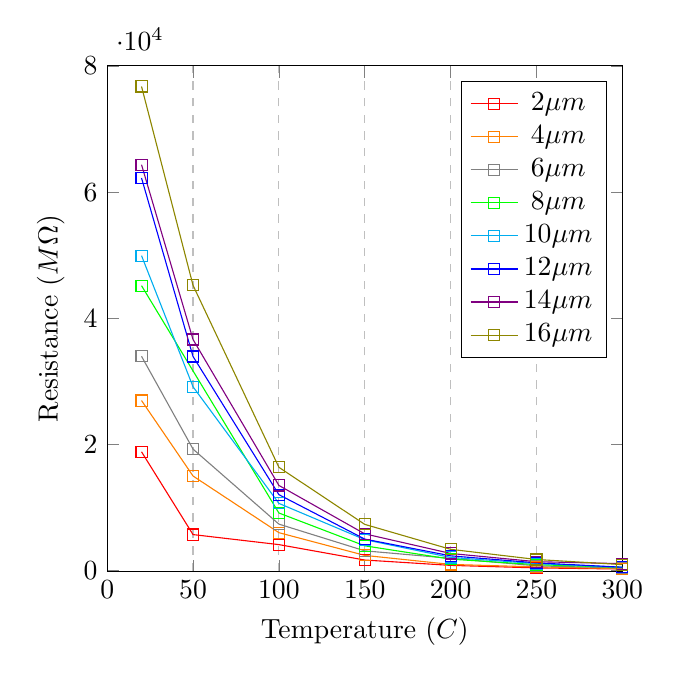
\begin{tikzpicture}

\begin{axis}[
    %title={Temperature dependence of CuSO$_4\cdot$5H$_2$O solubility},
    xlabel={Temperature ($\degree C$)},
    ylabel={Resistance ($M\Omega$)},
    height=8cm,
    width=0.67\textwidth,
    xmin=0, xmax=300,
    ymin=-100, ymax=80000,
    xtick={0, 50, 100, 150, 200, 250, 300},
    ytick={0,  20000, 40000, 60000, 80000},
    legend pos=north east,
    xmajorgrids=true,
    grid style=dashed,
]

\addplot[color=red, mark=square]
  coordinates {
    (20, 18838.831960510532)
    (50, 5721.196433673935)
    (100, 4132.0621710296264)
    (150, 1688.6948729656475)
    (200, 841.2150433392334)
    (250, 440.302012013769)
    (300, 261.4060018956609)
};
  \addlegendentry{$2\mu m$}


\addplot[color=orange, mark=square]
  coordinates {
    (20, 26964.56993084825)
    (50, 15004.623550776592)
    (100, 6024.400680383666)
    (150, 2421.909455798071)
    (200, 992.941517798109)
    (250, 599.1596921388986)
    (300, 324.22323501576)
};
  \addlegendentry{$4\mu m$}


  \addplot[color=gray, mark=square]
    coordinates {
      (20, 33975.32366479772)
      (50, 19267.82820081145)
      (100, 7380.478224259595)
      (150, 3145.40200426434) % still waiting on 200C for 6um
      (250, 769.1633331672097)
      (300, 422.36582758678955)
  };
    \addlegendentry{$6\mu m$}


  \addplot[color=green, mark=square]
    coordinates {
      (20, 45171.37333137492) % 50C is an abnormal result
      (100, 9142.39378668232)
      (150, 3940.371048004494)
      (200, 1831.0044653288925)
      (250, 955.8715312298274)
      (300, 520.5559254545812)
  };
    \addlegendentry{$8\mu m$}

    \addplot[color=cyan, mark=square]
      coordinates {
        (20, 49929.99691362574)
        (50, 29143.23401685659)
        (100, 10665.415563594671)
        (150, 4916.773356381926)
        (200, 2097.9457181960645)
        (250, 1126.8803002926064)
        (300, 544.5807811785508)
    };
      \addlegendentry{$10\mu m$}

  \addplot[color=blue, mark=square]
        coordinates {
          (20, 62233.17446628794)
          (50, 33945.186271498425)
          (100, 12048.750307108248)
          (150, 5005.786825762101)
          (200, 2353.3087715880146)
          (250, 1239.3991541526978)
          (300, 549.4831148923541)
      };
        \addlegendentry{$12\mu m$}

        \addplot[color=violet, mark=square]
          coordinates {
            (20, 64344.37794965449)
            (50, 36636.84609274838)
            (100, 13512.470055720295)
            (150, 5836.263210347023)
            (200, 2730.433679466901)
            (250, 1425.1543189284148)
            (300, 1113.215991329854)
        };
          \addlegendentry{$14\mu m$}

  \addplot[color=olive, mark=square]
      coordinates {
          (20, 76743.34343713324)
          (50, 45219.66140847825)
          (100, 16382.420423862137)
          (150, 7338.793759028416)
          (200, 3385.7192576547885)
          (250, 1774.7713800596902)
          (300, 960.6249944068636)
          };
    \addlegendentry{$16\mu m$}

\end{axis}
\end{tikzpicture}

\caption{Plot of Resistance vs Temperature on Substrate A for different Gap Sizes, including resistance from contacts}
\label{fig:results:res_temp_w_contacts}
\end{center}
\end{figure}
